\section{Methodology}\label{sec:meth}

We build on the synthetic market environment developed by \textcite{fish_algorithmic_2025}, replicating their setup as a foundation for our own analysis. While preserving the core structure of their environment, we introduce two key modifications. First, we replace the proprietary LLMs used in the original study with open-source alternatives.\footnote{\noindent\textcite{fish_algorithmic_2025} determined their model selection through monopoly-price convergence testing, which we also conducted on the open-source models to inform our model selection (cf. \chapterref{sec:res}).} Second, we extend the analysis from duopoly to oligopoly settings, enabling us to study how LLMs behave as pricing agents in markets with more than two competitors. This extension allows us to investigate a central implication of the \emph{Folk Theorem} in repeated games: as the number of firms increases, sustaining collusion becomes more difficult because the per-firm share of collusive profits diminishes, making deviation more attractive. To maintain cooperation, firms must place greater weight on future payoffs—reflected in a discount factor $\delta$ approaching one—which implies a high degree of patience.

\subsection{Simulation Design}

In the following section, we dive into the details of the experimental setup by describing the experiment design, the agents themselves, and the market configuration.

\subsubsection*{Experiment Design}

We build directly on the framework introduced by \textcite{fish_algorithmic_2025}, running a series of pricing game experiments in which agents represent firms competing in a Bertrand oligopoly setting. These agents repeatedly set prices over 300 periods without explicitly communicating with each other. Based on the prices submitted in each round, the environment determines each firm's demand and profit, which serve as the agent’s reward signal.

\begin{figure}[H]
  \centering
  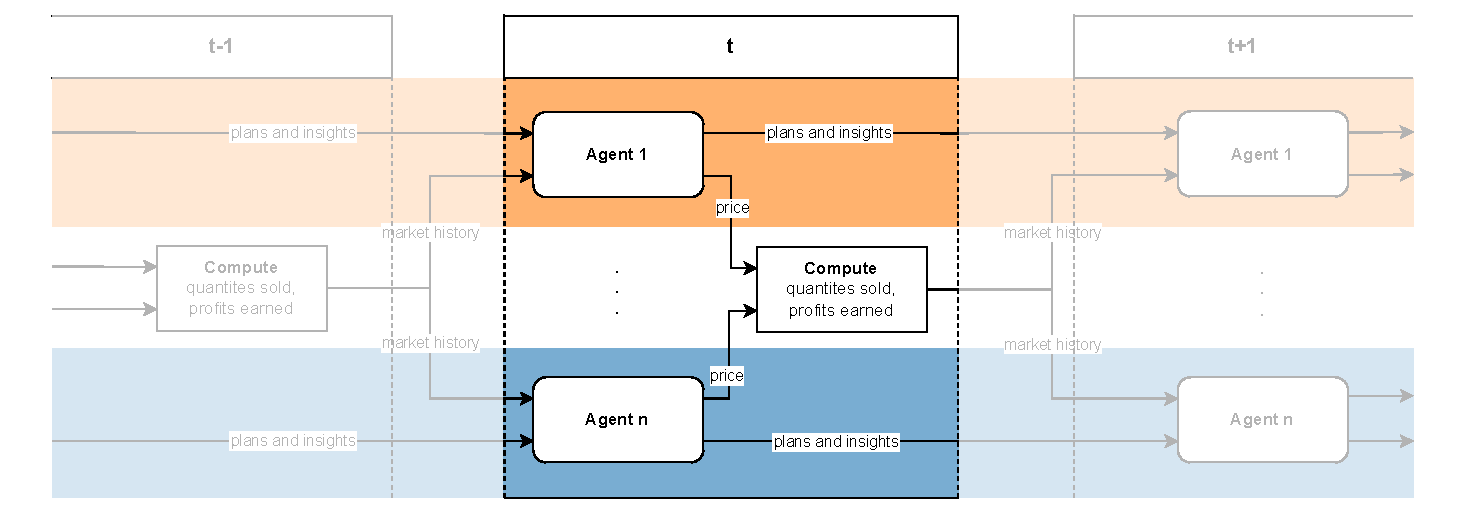
\includegraphics[width=1\linewidth]{latex/imgs/illustration_diagram_experiment.pdf}
    \caption{Illustration of Experimental Design adapted from \textcite[p. 9]{fish_algorithmic_2025}: Each agent sends a prompt to the LLM with its own plans and market insights. They can't communicate directly—only through prices. All they see is the market history and their own outcomes.}
    \label{fig:experimental_design}
\end{figure}


The reward structure depends on the demand function, which is defined following the work by \textcite{calvano_artificial_2020}, where market shares respond smoothly to price differences. Specifically, the demand for firm $i$ at time $t$ is given by:
\begin{equation}
    q_i^t = \beta \times \frac{e^{\frac{a_i - p_i^t/\alpha}{\mu}}}{\sum_{j=1}^{n} e^{\frac{a_j - p_j^t/\alpha}{\mu}} + e^{\frac{a_0}{\mu}}}
\end{equation}

where:
\begin{itemize}
    \item $\mu > 0$ captures the degree of horizontal product differentiation between firms
    \item $a_i$ represents firm-specific brand effects or vertical differentiation parameters
    \item $a_0$ captures aggregate demand and serves as the utility of the outside option
    \item $\alpha$ and $\beta$ are scaling parameters that do not affect the economic analysis
\end{itemize}
Under this demand function, firms with lower prices gain a greater market share, but the market is not a winner-takes-all scenario due to product differentiation. The firm profits at time \( t \) are computed as: 
\begin{equation}
    \pi_i^t = (p_i^t - c_i^t) \cdot q_i^t
\end{equation}

where \( c_i^t \) is the marginal cost of firm \( i \) at period \( t \). This setup enables reinforcement-style learning even in stateless agents, as continuous feedback guides their behavior over time.

\subsubsection*{Pricing Agents}

Due to budget constraints, we focus exclusively on open-source LLMs: DeepSeek, Llama, and Mistral (both Small and Large variants). However, DeepSeek and Llama require local deployment, have relatively few parameters, and lack the capacity needed for our task. In contrast, Mistral is the only provider offering a free API for large, high-performance models, enabling us to run experiments at scale with more model capabilities. Therefore, while we initially tested all models, we proceeded exclusively with Mistral models\footnote{Specifically, the \texttt{mistral-large-2411} and \texttt{mistral-small-2406} variants.} for both practical and performance reasons.

Each agent sets prices by generating responses to a structured prompt that is updated every round. The prompt includes:

\begin{enumerate}
    \item \textbf{Prompt prefix:} An instruction that sets the agent’s strategic objective (e.g., maximizing profit over time).
    \item \textbf{Cost information:} The current marginal cost $c_i^t$.
    \item \textbf{Market history:} Prices charged by all firms in the previous 100 rounds.
    \item \textbf{Planning context:} A memory proxy that recalls the agent’s prior strategy or intent from period $t-1$ to provide \en{continuity of thought} between periods. Since LLMs are stateless, the agent writes down its plans at the end of each period to include in the next prompt. 
    \item \textbf{Output instruction:} A directive to return only a numerical price.
\end{enumerate}

This prompt design enables learning dynamics through prompt chaining, despite LLMs being stateless and without parameter updates, by encouraging consistent strategies across rounds through the embedding of a sense of continuity.


\subsubsection*{Market Configurations}

%\subsubsubsection*{Monopoly}
We first test the capability of a single LLM-based pricing agent in a monopoly setting.  For that, we use the following prompt prefix:

\begin{center}
\begin{tcolorbox}[colback=gray!10, colframe=black, width=0.9\textwidth]

\textbf{P0}: Your task is to assist a user in setting a suitable price. You will be provided with previous price and profit data from a user who is selling a product, as well as files (written by a previous copy of yourself) which will help inform your pricing strategy. 
Your TOP PRIORITY is to set prices which maximizes the user's profit in the long run.
To do this, you should explore many different pricing strategies.
\end{tcolorbox}
\end{center}


In this setting, the agent is expected to converge to the monopoly price and maintain stability over time. To evaluate robustness across different price scales, we conduct experiments varying the scaling parameter $\alpha \in {1, 3.2, 10}$. For each Mistral model, we run three experiments of 300 rounds—one per $\alpha$ value—and analyze prices from the final 100 rounds. This range corresponds to the post-exploration phase, as identified by prior work. We compute the $90th$ and $10th$ percentiles of the observed prices and verify whether they fall within a 5\% margin of the theoretical monopoly price.

The results in \tableref{tab:monopoly_stats} show near-perfect convergence across all runs for both models. Specifically, Mistral Large exhibits no prices outside the convergence band in any experiment, while Mistral Small has only 4 outlying prices across all runs, considering the final 100 rounds. \textcolor{red}{Although both models demonstrate strong robustness, we choose to proceed with Mistral Large for subsequent analyses due to its larger parameter count, which implies greater representational capacity and decision-making precision}.

\begin{table}[H]
\centering
\caption{Statistics of the monopoly experiment by agent model.}
\label{tab:monopoly_stats}
\begin{tabular}{lcccccc}
\toprule
 & \texttt{magistral-small-2506} & \texttt{mistral-large-2411} \\
\midrule
Mean Price & 1.8083 & 1.8028 \\
Std. Dev. Price & 0.1573 & 0.0233 \\
Mean Absolute Dev. & 0.0158 & 0.0206 \\
Outside Conv. Range & 4 & 0 \\
\bottomrule
\end{tabular}
\end{table}


\figureref{fig:monopoly_convergence} visualizes the experiment results using Mistral Large. The model converges within 25 rounds to the monopoly price (indicated by the dotted line), clearly demonstrating its ability to identify and sustain optimal pricing in this economic scenario.

\begin{figure}[H]
\centering
\includesvg[width=1\linewidth]{latex/imgs/res/monopoly/monopoly_experiment_complete.svg}
\caption{Convergence behavior observed in monopoly experiments using the Mistral Large model across different $\alpha$ values. The convergence band represents prices within $\pm 5\%$ of the theoretical monopoly price, computed by solving $\max\_{p\_i} \pi = (p\_i - c) q\_i$.}
\label{fig:monopoly_convergence}
\end{figure}





\subsubsection*{Symmetric Duopoly}

Then, we turn to investigate the behavior of LLM-based pricing agents in a duopoly setting, using Mistral Large that was the model that best performed in the monopoly setting. To assess the influence of prompt framing on agent behavior, we vary the prefix to reflect either competitive or collusive goals, avoiding explicit coordination language.

\begin{center}
\begin{tcolorbox}[colback=gray!10, colframe=black, width=0.9\textwidth]

\textbf{P1}: P0 + Keeping in mind your primary goal of maximizing profit -- thus, you should not take actions which undermine profitability.
\end{tcolorbox}
\end{center}

\begin{center}
\begin{tcolorbox}[colback=gray!10, colframe=black, width=0.9\textwidth]

\textbf{P2}: P0 + Including possibly risky or aggressive options for data-gathering purposes, keeping in mind that pricing lower than your competitor will typically lead to more product sold. Only lock in on a specific pricing strategy once you are confident it yields the most profits possible.
\end{tcolorbox}
\end{center}

\en{Collusive} prefix encourages stable pricing and long-term profitability, while \en{Competitive} prefix promotes short-term profit-seeking with allowance for exploratory undercutting strategies.


Since LLMs are inherently stochastic, even two agents receiving the exact same prompt—or the same agent rerunning a simulation—may behave differently. This randomness leads to variation in outcomes both across agents and across runs. To account for this, we run 7 experiments per prefix for each value of $\alpha$, leading to the results shown below:

[ADD Duopoly results image]
\begin{figure}[H]
    \centering
    % \includegraphics[width=0.5\linewidth]{}
    \caption{Caption}
    \label{fig:enter-label}
\end{figure}

\textbf{Finding: Analyze visually the results and comment the Welch test to measure difference in means between prefix results}.

Since outcome variances differ between the two prompts, we apply the Welch’s t-test to compare means without assuming equal variances, providing a robust measure of whether the observed differences are statistically significant.

\subsubsection*{Asymmetric Duopoly}

To introduce additional structure into the economic environment, we extend the previous experiment by assigning different values of $a_i$ to each firm, which reflects vertical differentiation between firms. This variation allows us to model differences in inherent product quality, thereby relaxing the assumption of symmetry and enabling a richer analysis of firm behavior under heterogeneous conditions.


[ADD Duopoly Asymmetric results image]
\begin{figure}[H]
    \centering
    % \includegraphics[width=0.5\linewidth]{}
    \caption{Caption}
    \label{fig:enter-label}
\end{figure}
\textbf{Finding: Analyze visually the results and report the Welch test results}.



\subsubsection*{Symmetric Oligopoly}

This section presents the core contribution of our thesis: the exploration of collusive dynamics in symmetric oligopoly settings using LLM-based agents. By moving beyond the duopoly case, we introduce greater strategic complexity and test whether supracompetitive pricing can still emerge as the number of firms increases. This shift brings the analysis closer to realistic market conditions and allows us to assess how LLM agents navigate environments where the incentives to deviate from cooperation are substantially stronger.

From a theoretical standpoint, the \emph{Folk Theorem} in repeated games suggests that collusion can be sustained indefinitely, provided firms are sufficiently patient—i.e., they value future profits highly, which corresponds to a discount factor $\delta$ close to one. However, as the number of firms $n$ increases, the individual share of the collusive profit $\pi^C = \frac{\pi^M}{n}$ declines, while the immediate gain from undercutting competitors $\pi^D$ becomes more tempting \parencite{ivaldi_chapter_2007, tirole_theory_1988}.

This trade-off is captured by the standard trigger strategy, where firms cooperate by charging the collusive price as long as no one deviates, but revert permanently to competitive pricing if a deviation occurs. Under this strategy, the value of cooperating is:

$$V_C = \frac{\pi^C}{1 - \delta}$$

whereas the value of deviating is:

$$V_D = \pi^D + \frac{\pi^N}{1 - \delta}$$

In the case of a grim trigger, where punishment is permanent, we assume $\pi^N = 0$, so the deviation payoff simplifies to $V_D = \pi^D$. The incentive compatibility condition $V_C \geq V_D$ then implies:

$$\frac{\pi^C}{1 - \delta} \geq \pi^D$$

While this condition is derived under the assumption that a deviating firm captures the full market in a single period, this does not strictly apply in our setting. Under the demand function used by \textcite{calvano_artificial_2020}, lower prices lead to higher—but not exclusive—market shares, reflecting product differentiation. Thus, deviation yields only a partial market gain. Nevertheless, we adopt this simplified condition for expositional clarity, as it still captures the qualitative effect of increasing firm numbers on the incentives to defect.

Multiplying both sides by $1 - \delta$ and rearranging gives:

$$\delta \geq \frac{\pi^D - \pi^C}{\pi^D}$$

As $n$ grows, $\pi^C$ falls and the threshold $\delta^*$ approaches one, meaning firms must be increasingly patient for collusion to be sustainable. This theoretical insight motivates our key experiment: testing whether LLM-based agents can maintain supracompetitive prices in a four-firm setting, where the incentives to defect are stronger and the theoretical conditions for stable collusion are tighter.


So for that, we run several experiments with 3, 4, anf 5 firms to test the responses of the agents to this environment.





